\subsection{Database and Settings}
We consider the AR database~\cite{Martinez_CVC1998} for evaluation, which contains 126 individuals with more than 4000 frontal face images. In our experiment, we consider a subset of AR by randomly choosing 100 individuals with 50 men and 50 women. All images are converted into grayscale. We crop and rescale the images into 96$\times$96 and 24$\times$24 pixels as HR and LR images, respectively. For each subject in AR, we only consider the neutral image and images with expression variations from Session 1 in the training set. The remaining ones in both sessions are viewed as test images.
%figure 5
\begin{figure}
\graphicspath{{fig/}}
        \begin{center}
            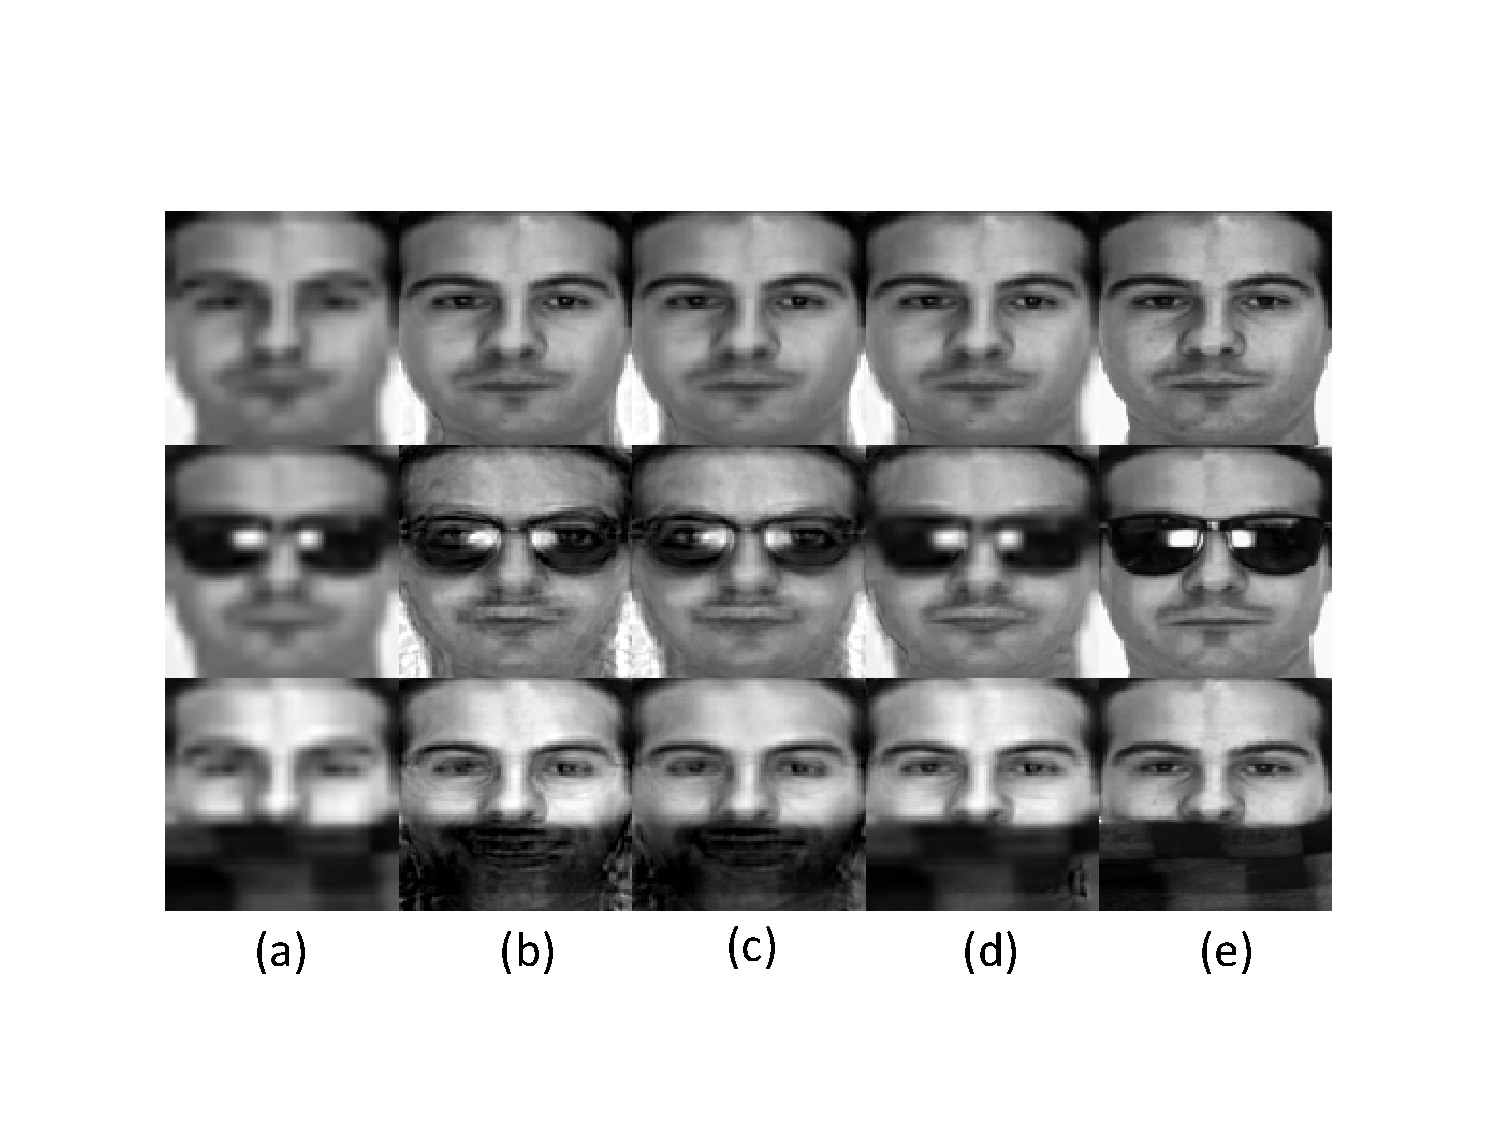
\includegraphics[scale=0.32]{exp_ori.pdf}
            \vspace{-0.3cm}
            \caption{\small{Example face hallucination results including occluded image regions. Images in each row are outputs of (a) Bicubic, (b) Jung \emph{et al.}~\cite{convex}, (c) Jiang \emph{et al.}~\cite{Jiang_TMM2014}, (d) ours, and (e) the ground truth.} \label{fig:exp_ori}}
        \end{center}\vspace{-.5cm}
\end{figure}

% table1
\begin{table}
\small
\renewcommand{\arraystretch}{1.2}
\centering
\caption{\small{Comparisons of average PSNR \& SSIM values of face hallucination outputs with occlusion.}}\label{tab:partA}
\vspace{0.2cm}
\begin{tabular}{|c|c|c|c|c|}
\hline
 & Bicubic & \cite{convex} & \cite{Jiang_TMM2014}  & Ours\\
\hline
PSNR  & 24.09 & 23.67 & 24.05 & \textbf{24.58}\\
\hline
SSIM  & 0.7975 & 0.7240 & 0.7404 & \textbf{0.8094}\\
\hline
\end{tabular}\vspace{-.3cm}
\end{table}

\subsection{Face Hallucination}

To evaluate our face hallucination results, we consider the LR face image inputs with and without occlusion. In addition, since our method is able to identify the corrupted pixels automatically, we further include the evaluation of recovered HR images using non-occluded pixels only. This is to show that, after disregarding such undesirable pixels, our method is able to achieve improved image quality for face hallucination.

We first compare the example outputs in Figure~\ref{fig:exp_ori}, in which the HR images (including the occluded image regions) are produced by bicubic, the approaches of \cite{convex} and \cite{Jiang_TMM2014}, and ours. In addition, we also show the ground truth HR images in the last column of Figure~\ref{fig:exp_ori}. From this figure, we see that our approach achieved satisfactory image quality for non-occluded image regions. Recall that our method views occluded regions as image corruption, and thus the corresponding pixels are produced by bicubic interpolation. In Table~\ref{tab:partA}, we quantitatively compare the image quality using PSNR and SSIM values. It can be seen that our approach was able to achieve improved results than other SR methods did.

Next, we consider the comparisons in which the HR images are corruption free. In other words, we apply our proposed method to remove the undesirable image pixels (mainly due to occlusion) from the HR images of different approaches. Figure~\ref{fig:exp_msk} and Table~\ref{tab:partB} present and compare the results of different approaches. We see that, after removing such corrupted image pixels, our method still obtained improved image quality for the remaining pixels of interest, and thus performed favorably against other SR approaches. Therefore, from the above qualitative and quantitative evaluation, the effectiveness of our proposed method for occlusion invariant face hallucination can be successfully verified.

%figure 6
\begin{figure}
\graphicspath{{fig/}}
        \begin{center}
            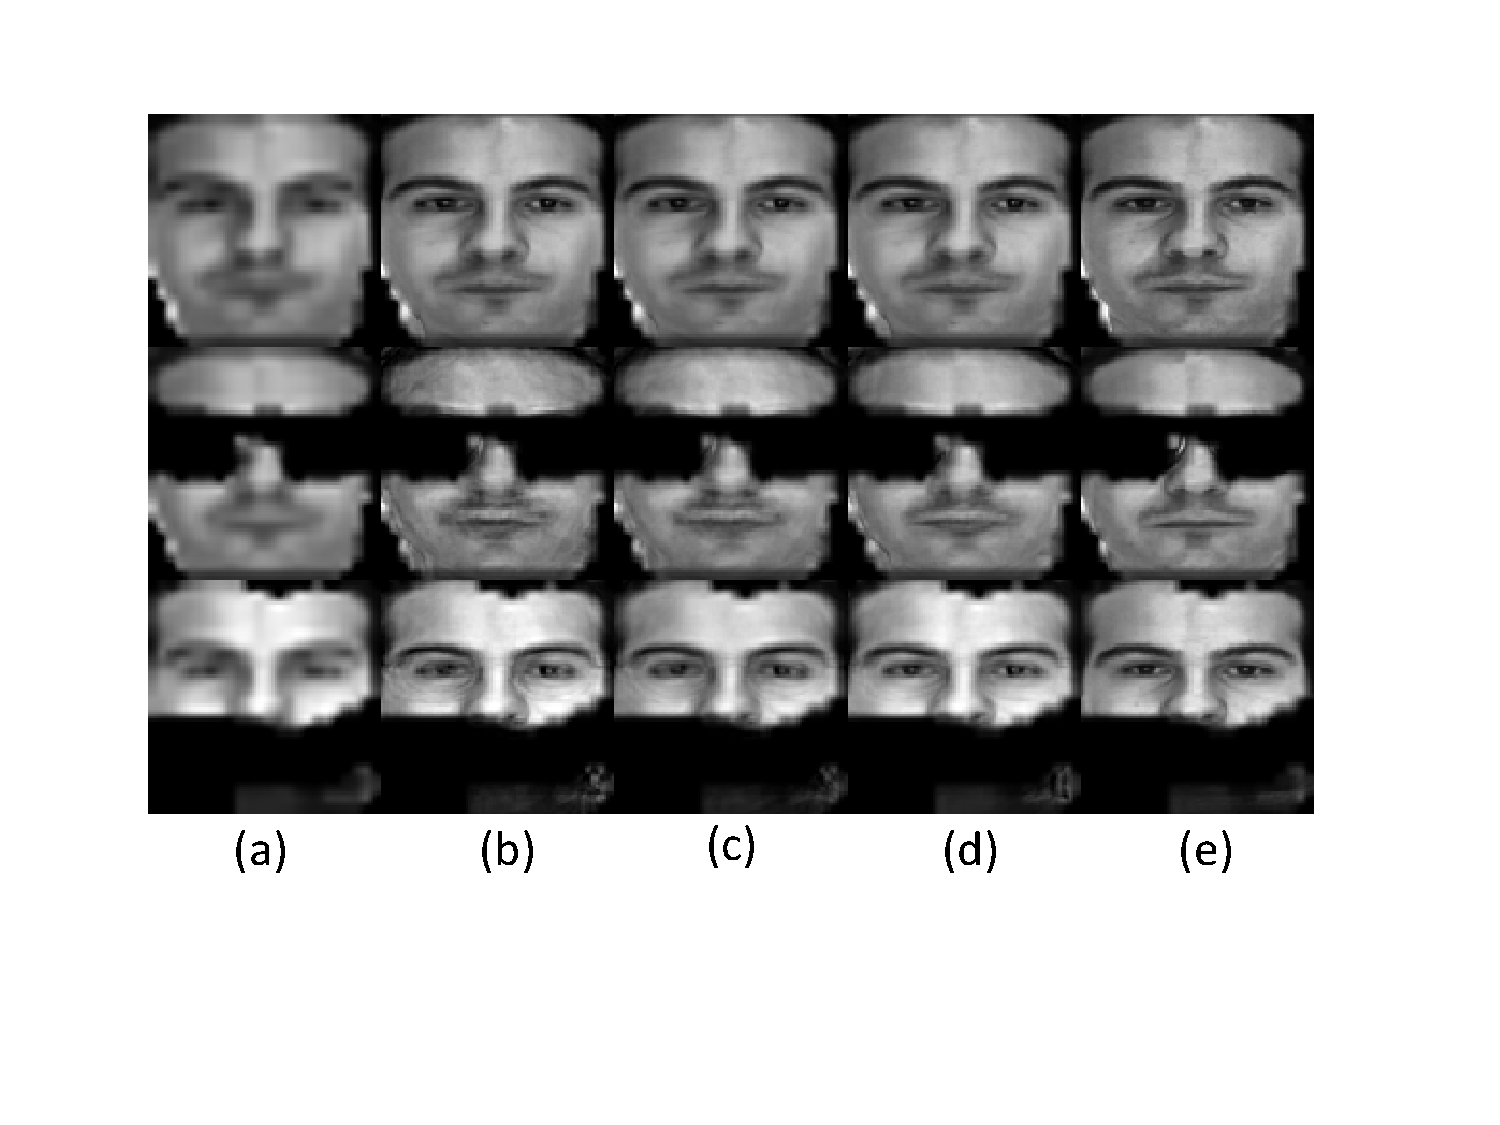
\includegraphics[scale=0.32]{exp_masked.pdf}
            \vspace{-0.3cm}
            \caption{\small{Example face hallucination results with corrupted pixels removed. Images in each row are outputs of (a) Bicubic, (b) Jung \emph{et al.}~\cite{convex}, (c) Jiang \emph{et al.}~\cite{Jiang_TMM2014}, (d) ours, and (e) the ground truth.} \label{fig:exp_msk}}
        \end{center}\vspace{-.5cm}
\end{figure}
%table 2
\begin{table}
\small
\renewcommand{\arraystretch}{1.2}
\centering
\caption{\small{Comparisons of average PSNR \& SSIM values of face hallucination outputs without corrupted pixels.}} \label{tab:partB}
\vspace{0.2cm}
\begin{tabular}{|l|c|c|c|c|}
\hline
 & Bicubic & \cite{convex} & \cite{Jiang_TMM2014}  & Ours\\
 \hline
PSNR  & 26.40 & 26.64 & 27.05 & \textbf{27.13}\\
\hline
SSIM  & 0.8659  & 0.8588  & 0.8672 & \textbf{0.8806}\\
\hline
\end{tabular}\vspace{-.3cm}
\end{table}


% table recog
\begin{table}[!t]
\small
\renewcommand{\arraystretch}{1.2}
\centering
\caption{\small{LR-to-HR recognition performance on AR.}}\label{tab:recog}\vspace{.2cm}
\begin{tabular}{|c|c|c|c|c|c|}
\hline
LR/LR & Bicubic & \cite{convex} & \cite{Jiang_TMM2014} & Ours & HR/HR\\
\hline
82.21 & 80.33 & 79.68 & 76.63 & 87.37 & 87.79\\
\hline
\end{tabular}
%\hline
%LR & HR Bicubic & HR by \cite{convex}\\
%\hline
%82.21 & 80.33 & 79.68\\
%\hline
%HR by \cite{Jiang_TMM2014} & HR by ours & HR\\
%\hline
%76.63 & 87.37 & 87.79\\
%\hline
%\begin{tabular}{lllll}
%\hline
%\multicolumn{1}{|c|}{Method}           & \multicolumn{1}{c|}{LR} & \multicolumn{1}{c|}{HR\_Bicubic} & \multicolumn{1}{c|}{HR by~\cite{convex}} & \multicolumn{1}{c|}{HR\_Ours} \\ \hline
%\multicolumn{1}{|c|}{Accuracy} & \multicolumn{1}{c|}{85.50} & \multicolumn{1}{c|}{80.33}          & \multicolumn{1}{c|}{83.50}       & \multicolumn{1}{c|}{88.50}       \\ \hline
%\end{tabular}\vspace{-.3cm}
\end{table}

\subsection{LR-to-HR Face Recognition}\vspace{-.1cm}

We now consider face recognition with LR images as test inputs, while \emph{only} the HR ones for training. This is to confirm that, in addition to improved HR outputs, our proposed method can be applied to LR-to-HR face recognition.

To recognize the LR images, we first apply our method to recover their HR versions. Next, the approach of sparse representation based classification (SRC) \cite{Wright_PAMI2009} will be applied to perform recognition. We note that, for comparison purposes, LR/LR (HR/HR) in Table~\ref{tab:recog} indicates the direct use of LR (HR) images for both training and testing. Their performances can be viewed as lower/upper bounds for recognition. In addition to bicubic interpolation, we also consider recent approaches of \cite{convex} and \cite{Jiang_TMM2014} to synthesize the HR outputs for recognition. Table~\ref{tab:recog} compares the recognition results of different methods. From this table, we see that our approach achieved the highest recognition rate, which supports the the use of our proposed scheme for LR-to-HR face recognition.




